% 图 5.14 CsCl 型 bcc 反铁磁三种结构（双胞块，角点+体心球，黑 +/白 −）
% 已对照原书 p.97 放大核读；原书面板无 (a)(b)(c) 标注
\documentclass[tikz,border=5pt]{standalone}
\usetikzlibrary{arrows.meta,calc}
\usepackage{amsmath}
\usepackage{bm}
\usepackage{fontspec}
\setmainfont{Times New Roman}
\newcommand\ball[2]{{%
  \ifnum#2>0
    \node[circle,fill=black,inner sep=0,minimum size=6.6pt] at (#1) {};
    \node[white,font=\tiny\bfseries,inner sep=0] at (#1) {$+$};
  \else
    \node[circle,fill=white,draw=black,line width=0.6,inner sep=0,minimum size=6.6pt] at (#1) {};
    \node[font=\tiny\bfseries,inner sep=0] at (#1) {$-$};
  \fi}}
\begin{document}
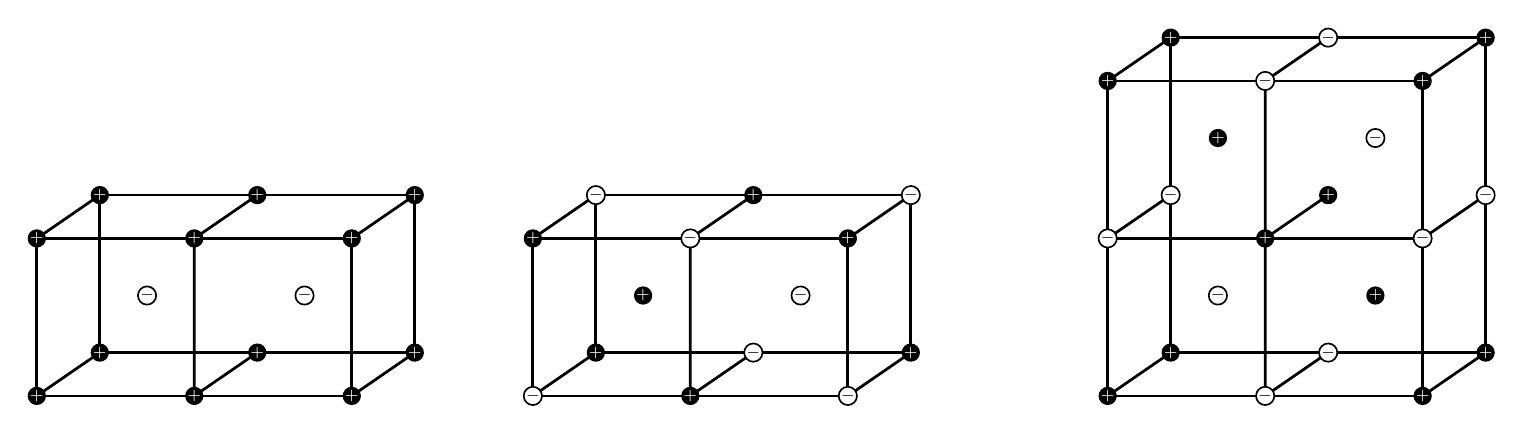
\begin{tikzpicture}[line width=0.8pt,>=Stealth]
% ---------- (a) 2x1x1: all corners +, body centres - ----------
\begin{scope}[shift={(0,0)}]
  \draw[line width=1.0] (0,2) -- (4,2) -- (4,0) -- (0,0) -- cycle;
  \draw[line width=1.0] (0.8,2.55) -- (4.8,2.55) -- (4.8,0.55) -- (0.8,0.55) -- cycle;
  \draw[line width=1.0] (2,0) -- (2,2) (0,2) -- (0.8,2.55) (2,2) -- (2.8,2.55)
        (4,2) -- (4.8,2.55) (0,0) -- (0.8,0.55) (2,0) -- (2.8,0.55) (4,0) -- (4.8,0.55);
  \foreach \p in {{0,0},{0,2},{2,0},{2,2},{4,0},{4,2}}{\ball{\p}{1}}
  \foreach \p in {{0.8,0.55},{2.8,0.55},{4.8,0.55},{0.8,2.55},{2.8,2.55},{4.8,2.55}}{\ball{\p}{1}}
  \ball{1.4,1.275}{-1}\ball{3.4,1.275}{-1}
\end{scope}
% ---------- (b) 2x1x1: checkerboard corners, alternating body centres ----------
\begin{scope}[shift={(6.3,0)}]
  \draw[line width=1.0] (0,2) -- (4,2) -- (4,0) -- (0,0) -- cycle;
  \draw[line width=1.0] (0.8,2.55) -- (4.8,2.55) -- (4.8,0.55) -- (0.8,0.55) -- cycle;
  \draw[line width=1.0] (2,0) -- (2,2) (0,2) -- (0.8,2.55) (2,2) -- (2.8,2.55)
        (4,2) -- (4.8,2.55) (0,0) -- (0.8,0.55) (2,0) -- (2.8,0.55) (4,0) -- (4.8,0.55);
  \ball{0,2}{1}\ball{2,2}{-1}\ball{4,2}{1}
  \ball{0,0}{-1}\ball{2,0}{1}\ball{4,0}{-1}
  \ball{0.8,2.55}{-1}\ball{2.8,2.55}{1}\ball{4.8,2.55}{-1}
  \ball{0.8,0.55}{1}\ball{2.8,0.55}{-1}\ball{4.8,0.55}{1}
  \ball{1.4,1.275}{1}\ball{3.4,1.275}{-1}
\end{scope}
% ---------- (c) 2x2x1: vertical period doubling + in-plane checkerboard ----------
\begin{scope}[shift={(13.6,0)}]
  \draw[line width=1.0] (0,4) -- (4,4) -- (4,0) -- (0,0) -- cycle;
  \draw[line width=1.0] (0.8,4.55) -- (4.8,4.55) -- (4.8,0.55) -- (0.8,0.55) -- cycle;
  \draw[line width=1.0] (0,2) -- (4,2) (2,0) -- (2,4)
        (0,4) -- (0.8,4.55) (2,4) -- (2.8,4.55) (4,4) -- (4.8,4.55)
        (0,2) -- (0.8,2.55) (2,2) -- (2.8,2.55) (4,2) -- (4.8,2.55)
        (0,0) -- (0.8,0.55) (2,0) -- (2.8,0.55) (4,0) -- (4.8,0.55);
  \ball{0,4}{1}\ball{2,4}{-1}\ball{4,4}{1}
  \ball{0,2}{-1}\ball{2,2}{1}\ball{4,2}{-1}
  \ball{0,0}{1}\ball{2,0}{-1}\ball{4,0}{1}
  \ball{0.8,4.55}{1}\ball{2.8,4.55}{-1}\ball{4.8,4.55}{1}
  \ball{0.8,2.55}{-1}\ball{2.8,2.55}{1}\ball{4.8,2.55}{-1}
  \ball{0.8,0.55}{1}\ball{2.8,0.55}{-1}\ball{4.8,0.55}{1}
  \ball{1.4,3.275}{1}\ball{3.4,3.275}{-1}
  \ball{1.4,1.275}{-1}\ball{3.4,1.275}{1}
\end{scope}
\end{tikzpicture}
\end{document}
